\documentclass[12pt]{article}
\usepackage{amsmath}
\usepackage{amssymb}
\usepackage[letterpaper,margin=0.85in,centering]{geometry}
\usepackage{fancyhdr}
\usepackage{enumerate}
\usepackage{lastpage}
\usepackage{multicol}
\usepackage{graphicx}

\reversemarginpar

\pagestyle{fancy}
\cfoot{Page \thepage \ of \pageref{LastPage}}\rfoot{{\bf Total Points: 40}}
\chead{MATH 4310}\lhead{Term Test II}\rhead{Monday, 17\textsuperscript{th} November, 2014}

\newcommand{\points}[1]{\marginpar{\hspace{24pt}[#1]}}
\newcommand{\skipline}{\vspace{12pt}}
%\renewcommand{\headrulewidth}{0in}
\headheight 30pt

\newcommand{\di}{\displaystyle}
\newcommand{\R}{\mathbb{R}}
\newcommand{\N}{\mathbb{N}}
\newcommand{\Z}{\mathbb{Z}}
\newcommand{\abs}[1]{\lvert #1\rvert}

\begin{document}

\author{Instructor: Sean Fitzpatrick}
\thispagestyle{plain}
\begin{center}
\emph{University of Lethbridge}\\
Department of Mathematics and Computer Science\\
17\textsuperscript{th} November, 2014, 5:00-5:50 pm\\
{\bf Math 4310 - Term Test II}\\
\end{center}
Last Name:\underline{\hspace{50pt}{\bf SOLUTIONS}\hspace{50pt}}\\
\skipline
First Name:\underline{\hspace{50pt}{\bf THE}\hspace{100pt}}\\
\skipline
Student Number:\underline{\hspace{322pt}}\\


\vspace{0.5in}


\begin{quote}
 {\bf Record your answers below each question in the space provided.    Left-hand pages may be used as scrap paper for rough work.  If you want any work on the left-hand pages to be graded, please indicate so on the right-hand page.
 
 \bigskip
 
Partial credit will be awarded for partially correct work, so be sure to show your work, and include all necessary justifications needed to support your arguments. 
}
\end{quote}


\vspace{0.5in}

For grader's use only:

\begin{table}[hbt]
\begin{center}
\begin{tabular}{|l|r|} \hline
Page&Grade\\
\hline \hline
\cline{1-2} 2 & \enspace\enspace\enspace\enspace\enspace\enspace/12\\
\cline{1-2} 3 & \enspace\enspace\enspace\enspace\enspace\enspace/8\\
\cline{1-2} 4 & \enspace\enspace\enspace\enspace\enspace\enspace/10\\
\cline{1-2} 5 & \enspace\enspace\enspace\enspace\enspace\enspace/10\\
\cline{1-2} Total & \enspace\enspace\enspace\enspace\enspace\enspace/40\\
\hline
\end{tabular}

\skipline

\skipline

\skipline


\end{center}
\end{table}
\newpage


\begin{enumerate}
\item Let $X$ be a topological space. List as many conditions as possible equivalent to the statement ``$X$ is not connected.'' \points{6} You don't need to justify your responses.

(Note: It is possible to earn bonus points on this problem. I will give 2 points per correct response, up to 6 points, plus 1 point for any additional correct responses.)

\bigskip

Here I was looking for answers that (a) didn't depend on $X$ being a particular type of space, and (b) were {\em equivalent} in the sense of ``$X$ is not connected if and only if...'' and were more interesting than ``$X$ is homeomorphic to $Y$ and $Y$ is not connected.'' Possible responses included:
\begin{itemize}
 \item There exists a continuous surjection $f:X\to \{0,1\}$.
 \item There exist nonempty, open, disjoint sets $U,V\subseteq X$ such that $X=U\cup V$.
 \item There exist nonempty disjoint sets $A,B\subseteq X$ such that $X=A\cup B$, and $A\cap \overline{B} = \overline{A}\cap B = \emptyset$.
 \item There exists a proper nonempty subset $A\subseteq X$ that is both open and closed in $X$.
 \item There exists a proper nonempty subset $A\subseteq X$ with $\partial A = \emptyset$.
\end{itemize}

\bigskip

\item Let $X$ be a subspace of $\R^n$ (with the Euclidean topology). List as many conditions as possible equivalent to the statement ``$X$ is compact.'' \points{6} The same scoring rules apply as in Problem \#1.


\bigskip

With the same expectations as the previous problem, $X$ is a compact subspace of $\R^n$ if and only if
\begin{itemize}
 \item Every open cover of $X$ admits a finite subcover.
 \item $X$ is closed and bounded.
 \item Any infinite subset of $X$ has a limit point.
 \item Any sequence in $X$ has a convergent subsequence.
\end{itemize}
(Note that except for the first point, the other three depend on $X$ being a subspace of Euclidean space.)

\newpage

\item Let $X$ and $Y$ be topological spaces, where $X$ is compact and $Y$ is Hausdorff, and let $f:X\to Y$ be continuous.
\begin{enumerate}
 \item Prove that if $f:X\to Y$ is a surjection, then $f$ is a quotient map. \points{5}

\bigskip

It suffices to prove that $f$ is a closed map, since if $f^{-1}(A)$ is closed in $X$ for some subset $A\subseteq Y$, then since $f$ is a surjection we have that $f(f^{-1}(A))=A$ is closed in $Y$. (If $f$ was not a surjection we would only have $f(f^{-1}(A))\subseteq A$.) It follows that $f^{-1}(A)$ is closed if and only if $A$ is closed, and by taking complements this is equivalent to the requirement that $f^{-1}(A)$ is open if and only if $A$ is open.

Now, suppose that $F\subseteq X$ is closed. Since $X$ is compact, $F$ must also be compact. Since $f$ is continuous, $f(F)$ is a compact subset of $Y$. Since $Y$ is Hausdorff, $f(F)$ is closed. Thus $f$ takes closed sets to closed sets, and therefore $f$ is a quotient map.

\bigskip

 \item Prove that if $f:X\to Y$ is a bijection, then $f$ is a homeomorphism. \points{3}

\bigskip

Since $f$ is a continuous bijection, it remains to show that $f^{-1}$ is continuous. From part (a) we know that $f$ is a closed map. Thus, if $A\subseteq X$ is closed, then $(f^{-1})^{-1}(A) = f(A)$ is closed in $Y$, so $f^{-1}$ is continuous.

\end{enumerate}
\newpage
 \item Prove that if $f:X\to Y$ is a continuous surjection and $X$ is path-connected, then $Y$ is path-connected. \points{5}

\bigskip

Suppose $X$ is path connected and let $f:X\to Y$ be a continuous surjection. Choose any points $y_0,y_1\in Y$. Since $f$ is onto, there exist points $x_0,x_1$ in $X$ with $f(x_0)=y_0$ and $f(x_1)=y_1$. Since $X$ is path-connected, there exists a path $\gamma:[0,1]\to X$ with $\gamma(0)=x_0$ and $\gamma(1)=x_1$, and then $f\circ\gamma:[0,1]\to Y$ is path in $Y$ with $f\circ\gamma(0)=f(x_0)=y_0$ and $f\circ\gamma(1)=f(x_1)=y_1$. Thus, $Y$ is path-connected.

\bigskip

 \item Suppose that $X=A\cup B$, with $A,B$ nonempty, disjoint, open subsets of $X$. (That is, $\{A,B\}$ is a separation of $X$.) Prove that a map $f:X\to Y$ is continuous if and only if the restrictions $f|_A:A\to Y$ and $f|_B:B\to Y$ are continuous. \points{5}

\bigskip

If $f:X\to Y$ is continuous, then the restrictions $f|_A$ and $f|_B$ are continuous, since restrictions are always continuous. (Recall that if $i_A:A\to X$ and $i_B:B\to X$ denote the inclusion maps, which are always continuous in the subspace topology, then $f|_A = f\circ i_A$ and $f|_B = f\circ i_B$.)

Now suppose that $f|_A:A\to Y$ and $f|_B:B\to Y$ are continuous. There are two approaches that work well here. One is to note that for any open subset $U\subseteq Y$, 
\[
(f|_A)^{-1}(U) = (f\circ i_A)^{-1}(U) = i_A^{-1}(f^{-1}(U)) = A\cap f^{-1}(U), 
\]
which is open in $X$, since $A$ and $f^{-1}(U)$ are open, and similarly $(f|_B)^{-1}(U) = B\cap f^{-1}(U)$ is open in $X$, so 
\[
 (A\cap f^{-1}(U))\cup (B\cap f^{-1}(U)) (A\cup B)\cap f^{-1}(U) = X\cap f^{-1}(U) = f^{-1}(U)
\]
is open in $X$, and thus $f$ is continuous. An alternative proof is to note that $f = (f|_A)\cup (f|_B):A\cup B\to Y$ and apply the gluing lemma, which holds trivially since $A\cap B = \emptyset$.

\newpage

 \item Suppose $\{F_n | n\in\N\}$ is a family of nonempty closed subsets of a topological space $X$, such that $F_{n+1}\subseteq F_n$ for each $n\in \N$. Prove that if $X$ is compact, then $\bigcap_{n\in\N}F_n$ is nonempty. \points{6}

Hint: To get a contradiction, suppose $\bigcap_{n\in\N}F_n = \emptyset$, and take complements.

 \bigskip

Suppose that $\bigcap_{n\in\N}F_n = \emptyset$. Then $X = \emptyset^c = \left(\bigcap_{n\in\N}F_n\right)^c = \bigcup_{n\in \N}F_n^c$, so the collection $\{F_n^c = X\setminus F_n : n\in\N\}$ is an open cover of $X$. Since $X$ is compact, there exists some finite subcover, so we can write
\[
 X = F_{n_1}^c\cup F_{n_2}^c\cup\cdots\cup F_{n_k}^c,
\]
where without loss of generality we assume $n_1<n_2<\cdots <n_k$. Since $F_{n+1}\subseteq F_n$ for all $n\in \N$, it follows that $F_m\subseteq F_n$ for all $m>n$, and thus $F_n^c\subseteq F_m^c$ for all $n<m$. Therefore we have $F_{n_1}^c\subseteq F_{n_2}^c\subseteq \cdots\subseteq F_{n_k}^c$, and thus $X = F_{n_k}^c$. But this implies that $F_{n_k}=\emptyset$, which is a contradiction, since all of the sets $F_n$ were assumed to be nonempty.

\bigskip

 \item Consider the cylinder $X=S^1\times [-1,1]$, and let $\sim$ be the equivalence relation on $X$ defined by the partition  $\mathcal{P}$ consisting of the sets $S^1\times\{-1\}$, $S^1\times\{1\}$, and the single point sets $\{(x,t)\}$, where $x\in S^1$ and $t\in (-1,1)$. Describe the quotient space $X/\sim$. \points{4} (A formal proof is not required.)

\bigskip

The quotient space corresponding to the given partition is obtained by collapsing the sets $X\times {1}$ and $X\times {-1}$ to a single point, and leaving all other points unaffected. If we collapsed only the set $X\times {1}$ to a point, we'd have a space homeomorphic to the cone $CS^1$, since $[0,1]$ is homeomorphic to $[-1,1]$. In this case we also collapse the bottom of the cone to a point, so the result is a ``double cone''. This space is known as the {\em suspension} of $S^1$; the suspension of any topological space is defined in the same manner. In the particular case of $S^1$ the suspension is also homeomorphic to the sphere $S^2$.
\begin{center}
 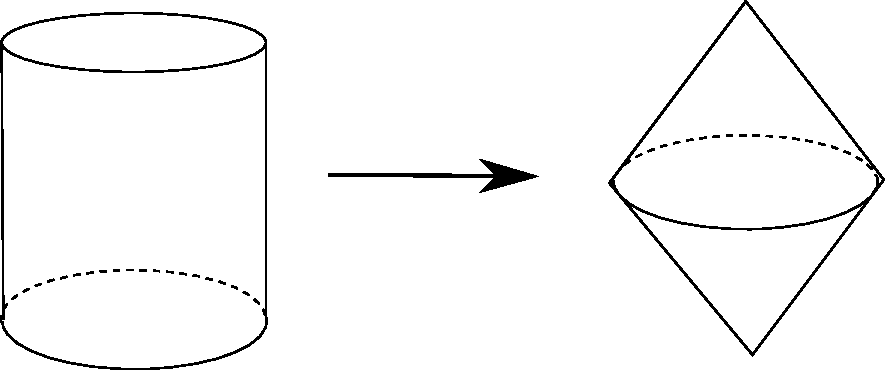
\includegraphics[width=4in]{Q7.pdf}
\end{center}

\end{enumerate}



\end{document}